\documentclass[10pt]{article}   % document properties
\usepackage[spanish]{babel}     % spanish package
\usepackage[utf8]{inputenc}     % codificacion de caracteres utf-8
\usepackage[top=2.3cm,bottom=3.5cm,right=2.5cm,left=2.5cm]{geometry}   % modify margins 
\usepackage{multicol}           % multiple columsn
\usepackage{graphicx}           % manage images 
\usepackage{url}                % manage aesthetic links
\usepackage{hyperref}           % internal links and more
\usepackage{array}              % customize tables         
%\usepackage{tcolorbox}          % colorful boxes
\usepackage{caption}            % improve figures & tables captions
\usepackage{tabularx}           % table advanced (sized)
\usepackage{lipsum}             % lipsum text
\usepackage{fancyhdr}           % headers and footers
\usepackage{xcolor, colortbl}   % define customize colors & table colore
\usepackage{listings}           % show & customize code
%%%%%%%%%%%%%%%%%%%%%%%%%%%%%%  extra definitions  %%%%%%%%%%%%%%%%%%%%%%%%%%%%%%%
\lstdefinestyle{ascii-tree}{
	literate={├}{|}1 {─}{--}1 {└}{+}1 
}
\newcolumntype{M}[1]{>{\centering\arraybackslash}m{#1}}     % cell configuration
\pagestyle{fancy}               % choosing fancy style
\fancyhf{}                      % delete any footer or header
\renewcommand{\headrulewidth}{0pt} % delete header line
% para el codigo fuente
\definecolor{dkgreen}{rgb}{0,0.6,0}
\definecolor{gray}{rgb}{0.5,0.5,0.5}
\definecolor{graya}{rgb}{0.97,0.97,0.97}
\definecolor{mauve}{rgb}{0.58,0,0.82}
\definecolor{codebackground}{rgb}{0.95, 0.95, 0.92}
\definecolor{tablebackground}{rgb}{0.8, 0, 0}
\lstset{
      frame=tb,
      language=bash,
      aboveskip=3mm,
      belowskip=3mm,
      showstringspaces=false,
      columns=flexible,
      basicstyle={\small\ttfamily},
      numbers=left,
      numberstyle=\tiny\color{gray},
      keywordstyle=\color{blue},
      commentstyle=\color{dkgreen},
      stringstyle=\color{mauve},
      breaklines=true,
      breakatwhitespace=true,
      tabsize=3,
      backgroundcolor= \color{codebackground}
}

%%%%%%%%%%%%%%%%%%%%%%%%%%%%%%%%%%%  variables  %%%%%%%%%%%%%%%%%%%%%%%%%%%%%%%
\newcommand{\itemCourse}{Programación Web 2}
\newcommand{\itemTheme}{Docker}
\newcommand{\itemPracticeNumber}{01}
\newcommand{\itemAcademic}{2024 - A}
\newcommand{\itemSemester}{III} %Romanos de preferencia
\newcommand{\itemDate}{05 / 05 / 2024}
\newcommand{\itemHour}{23:59 PM}

\newcommand{\itemStudentA}{Huayhua Hillpa Yourdyy Yossimar}
\newcommand{\itemStudentB}{Participante 2}
\newcommand{\itemStudentC}{Participante 3}
\newcommand{\itemStudentD}{Participante 4}

\newcommand{\itemTeacher}{Dr(a). Richart Smith Escobedo Quispe}
\newcommand{\itemUniversity}{Universidad Nacional de San Agustín de Arequipa}
\newcommand{\itemFaculty}{Facultad de Ingeniería de Producción y Servicios}
\newcommand{\itemDepartment}{Departamento Académico de Ingeniería de Sistemas e Informática}
\newcommand{\itemSchool}{Escuela Profesional de Ingeniería de Sistemas}
%%%%%%%%%%%%%%%%%%%%%%%%%%%%%%%%%%%   header  %%%%%%%%%%%%%%%%%%%%%%%%%%%%%%%%%%

\fancyhead[C]{
	\begin{tabularx}{\textwidth}{|M{3.8cm}|M{7.67cm}|M{3.8cm}|}
		\hline
		
\includegraphics[scale=0.45]{img/logo_episunsa.png} &\cellcolor{graya}{\textbf{\footnotesize\itemUniversity}\par\textbf{\footnotesize\itemFaculty}\par\textbf{\footnotesize\itemSchool}} & \vspace{0.16cm}
\includegraphics[scale=0.52]{img/logo_abet.png} \\
		\hline
		\multicolumn{3}{|c|}{\footnotesize \textbf{Formato:} Guía de Práctica de Laboratorio / Talleres / Centros de Simulación}\\
		\hline
		\cellcolor{graya}{\textbf{\footnotesize Aprobación: 2022/03/01}} & \textbf{\footnotesize Código: GUIA-PRLD-001} & \cellcolor{graya}{\textbf{\footnotesize Página: \thepage}} \\
		\hline
	\end{tabularx}}

\setlength{\headheight}{66pt}   % Ajusta la altura del encabezado
\setlength{\headsep}{16pt}      % Ajusta la separación entre el encabezado y el texto
\setlength{\footskip}{0pt}      % Ajusta la separación entre el final del texto y el pie de página

\begin{document}
    \vspace*{0cm}	
    \begin{center}	
        \fontsize{17}{17} \Large{\textbf{INFORME DE LABORATORIO}}
    \end{center}
    
    \begin{table}[h!]
        \renewcommand{\arraystretch}{1.7}
        \footnotesize
        \begin{tabular}{|m{2.4cm}|m{2.1cm}|m{2.4cm}|m{2cm}|m{2.64cm}|m{2.42cm}|}\hline 
            \rowcolor{tablebackground}
            \multicolumn{6}{|c|}{\textbf{\large\color{white} INFORMACION BASICA}}\\ \hline
            {\cellcolor{graya}{ASIGNATURA:}} & \multicolumn{5}{l|}{\itemCourse}\\ \hline 
            \cellcolor{graya}{TITULO DE LA PRACTICA:} & \multicolumn{5}{l|}{\itemTheme}\\ \hline 
            \cellcolor{graya}{NUMERO DE LA PRACTICA:} & \itemPracticeNumber & \cellcolor{graya}{AÑO LECTIVO:} & \itemAcademic & \cellcolor{graya}{N° SEMESTRE:} & \itemSemester\\ \hline 
            \cellcolor{graya}{FECHA DE \par PRESENTACION:} & \itemDate & \cellcolor{graya}{HORA DE \par PRESENTACION:} & \multicolumn{3}{l|}{\itemHour} \\ \hline 
            \multicolumn{4}{|l|}{\begin{minipage}{8cm}
                \vspace{0.5em}
                INTEGRANTE (s):
                \begin{itemize}
                    \setlength{\itemsep}{0pt}
                    \setlength{\parskip}{0pt}
                    \setlength{\parsep}{0pt}
                    \item \itemStudentA
                    %\item \itemStudentB
                    %\item \itemStudentC
                    %\item \itemStudentD
                \end{itemize}
                \vspace{0em} % Espaciado ajustable según necesidad
            \end{minipage}} & \cellcolor{graya}{NOTA:} & \\ \hline 
            \multicolumn{6}{|l|}{\begin{minipage}{8cm}
                \vspace{0.5em} % Espaciado ajustable según necesidad
                DOCENTE (s):
                \begin{itemize}
                    \setlength{\itemsep}{0pt}
                    \setlength{\parskip}{0pt}
                    \setlength{\parsep}{0pt}
                    \item \itemTeacher
                \end{itemize}
                \vspace{0em} % Espaciado ajustable según necesidad
            \end{minipage}}\\ \hline 	
        \end{tabular}
    \end{table}
    \normalsize
    
    \section{Proyecto Final de Programación web I}

El proyecto de programación web I consiste en la creación de una página web que permita la gestión de una tienda de productos. En este caso la aplicación web estaba orientada a una tienda de lentes, en la cual se podía realizar las siguientes acciones:
\begin{itemize}
    \item Registro de usuarios.
    \item Inicio de sesión.
    \item Visualización de productos.
    \item Administrar los pagina web (solo para el administrador).
    \item Comprar productos.
\end{itemize}

\subsection{Estructura del proyecto}

El proyecto se encuentra estruturado de la siguiente manera:
\clearpage

\begin{figure}[h]
    \centering
    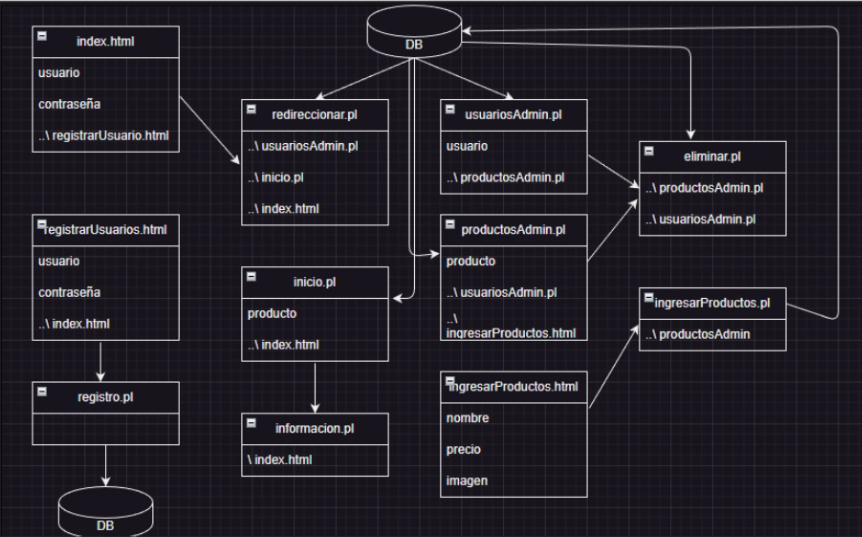
\includegraphics[width=0.8\textwidth,keepaspectratio]{img/estructura.png}
    %\includesvg{img/automata.svg}
    %\label{img:mot2}
    %\caption{Product backlog.}
\end{figure}

Para la elaboración del proyecto se utilizaron archivos Perl, para el envio de formularios, la escritura de documentos html y la conexion con la base de datos. Para el servidor local se utilizo una herramienta llamada Xampp.


\textbf{XAMPP: } es una distribución de Apache completamente gratuita y fácil de instalar que contiene MariaDB, PHP y Perl. El paquete de instalación de XAMPP ha sido diseñado para ser fácil de instalar y usar.

\section{El uso de Docker}

Para probar el funcionamiento del proyecto en docker, se instalo Docker Desktop. Luego se instalo la imagen de ubuntu para crear un contenedor para el proyecto. 

\begin{lstlisting}[language=bash,caption={Descargando la imagen de ubuntu}][H]
    > docker pull ubuntu
\end{lstlisting}

\begin{lstlisting}[language=bash,caption={Creando el contendor ubu}][H]
    > docker create --name ubu ubuntu
\end{lstlisting}

\begin{lstlisting}[language=bash,caption={Creando el contendor ubu}][H]
    > docker create -p8080:80 --name ubu ubuntu
\end{lstlisting}

\begin{lstlisting}[language=bash,caption={Inciando el servidor}][H]
    > docker start ubu
\end{lstlisting}

\begin{lstlisting}[language=bash,caption={Ingresamos al contenedor}][H]
    > docker exec -it ubu bash
\end{lstlisting}

\begin{lstlisting}[language=bash,caption={Instalando apache2 dentro del contenedor}][H]
    $ apt-get update
    $ apt-get install apache2
    $ a2enmod cgi
\end{lstlisting}

\begin{lstlisting}[language=bash,caption={Prendemos apache}][H]
    $ service apache2 start
\end{lstlisting}

\begin{lstlisting}[language=bash,caption={Se instala MariaDB y seguidamente lo activamos}][H]
    $ apt-get install mariadb-server
    $ service mariadb start
\end{lstlisting}

\begin{lstlisting}[language=bash,caption={Instalamos neovim para la edicion de archivos}][H]
    $ apt-get install neovim
\end{lstlisting}

Una vez que comprobamos que podemos usar la base de datos y el servidor apache, procedemos a copiar los archivos del proyecto al contenedor. Para ello se utilizo el comando \textbf{docker cp}.

\begin{lstlisting}[language=bash,caption={Copiando los archivos al contenedor}][H]
    > docker cp TrabajoFinalPweb1 ubu:/var/www/html
\end{lstlisting}

\begin{lstlisting}[language=bash,caption={Ingresamos al contenedor}][H]
    > docker exec -it ubu bash
\end{lstlisting}

Para que funcionen los archivos perl y cgi, tuve que mover los archivos a la carpeta /usr/lib/cgi-bin.

\begin{lstlisting}[language=bash,caption={Moviendo los archivos}][H]
    $ mv acciones/ comprar.cgi inicio.cgi registro.pl usuariosAdmin.pl catalogoAdmin.pl ingresarArticulos.html redireccionar.pl registroAdmin.pl /usr/lib/cgi-bin/
\end{lstlisting}

Luego en un archivo *.sql se insertaron los datos de la base de datos que tenia en XAMPP, para que luego los exporte a MariaDB en el contenedor.

\begin{lstlisting}[language=bash,caption={Exportando la base de datos}][H]
    $ mysql -u root -p < login.sql
\end{lstlisting}

Para configurar el el usuario y contraseña de la base de datos, se utilizo los siguientes comandos:

\begin{lstlisting}[language=bash,caption={Abriendo la configuración para establecer el usuario y contraseña}][H]
    $ service mariadb stop
    $ mysqld_safe --skip-grant-tables --skip-networking &
    $ mysql -u root
    $ FLUSH PRIVILEGES;
\end{lstlisting}

\begin{lstlisting}[language=bash,caption={Estableciendo el usuario y contraseña}][H]
    $ ALTER USER 'root'@'localhost' IDENTIFIED BY 'fangtastic';
\end{lstlisting}

\begin{lstlisting}[language=bash,caption={Reiniciando el servicio}][H]
    $ quit
    $ service mariadb restart
\end{lstlisting}

Al momento de poner a flote la aplicación web las paginas con terminación .cgi no funcionaban, por que en cada una se utilizaba una libreria que se instala con CPAN la cual es CGI::Ajax. Para instalarla trate de utilizar el siguiente comando: instal CGI::Ajax, pero no funciono. Por lo que tuve que quitar parte de la funcionalidad de la pagina web. 

Sin embargo aun queda una gran parte de ella. Esta se mostrara en el video de Youtube.

\section{URL's}
\begin{itemize}
    \item Video de Youtube: \url{https://youtu.be/qBstTw_4QxM}
\end{itemize}

\section*{REFERENCIAS}
\begin{itemize}
    \item XAMPP: \url{https://www.apachefriends.org/es/index.html}
    \item Docker Desktop: \url{https://www.docker.com/products/docker-desktop/}
\end{itemize}

 % Desarrolla tu contenido dentro de desarrollo
    %\input{conclusiones} % agregar las partes necesarias
    
\end{document}